\section{Más funcionalidades útiles}
\frame
{
\frametitle{pull}
\begin{itemize}
 \item \textbf{pull}\\ \indent
Utilizándolo sin ningún parámetro adicional -\textbf{git pull origin master}- funciona igual que un \textit{update} en Subversion. Es decir, se trae los cambios y hace \textit{merge}. Si le pasamos el parámetro \textit{-{}-rebase}, funciona como un \textit{rebase}.
\end{itemize}

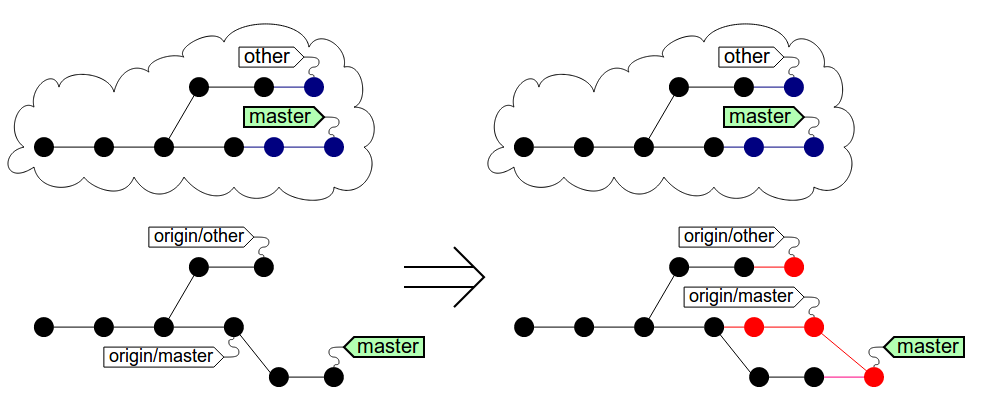
\includegraphics[height=5cm]{imgs/pull.png} 
}

\frame
{
\frametitle{ignore}
\begin{itemize}
 \item \textbf{gitignore}\\ \indent
Este fichero se suele colocar en la raíz del proyecto y el contenido suele ser un listado de elementos que no queremos que sean reconocidos como ficheros del repositorio. 
 \item \textbf{update-index -{}-assume-unchanged}\\ \indent
Este comando se utiliza para ficheros que accidentalmente se han \textit{comiteado} (y probablemente \textit{pusheado}) y no queremos tener en cuenta los cambios producidos en estos ficheros, ya que lo veremos como modificados en la etapa II (listo para \textit{comitear}).
\end{itemize}
}

\frame
{
\frametitle{revert}
\begin{itemize}
 \item \textbf{revert}\\ \indent
  Este comando deshace un único commit aplicando el parche con la diferencia como un nuevo commit. Ejemplo: git \textbf{revert} HEAD
 \begin{tabular}{p{4cm}|p{4cm}}\\
    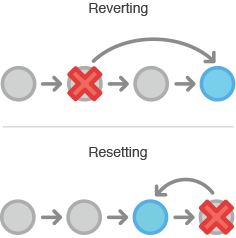
\includegraphics[height=4cm]{imgs/revert-vs-reset.png}&
    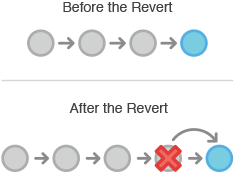
\includegraphics[height=3.5cm]{imgs/revert-sample.png}\\
 \end{tabular}
\end{itemize}

 Este comando no destruye la historia ni diverge las ramas \textit{master}. Ejemplo pack commits: git \textbf{revert} master\textasciitilde2..master
}

\frame
{
\frametitle{soft reset}
\begin{itemize}
 \item \textbf{soft reset}\\ \indent
 El comando git reset -{}-soft <hash> mueve el puntero de la cabeza al hash del commit que le indiquemos.\\
 \begin{center}
    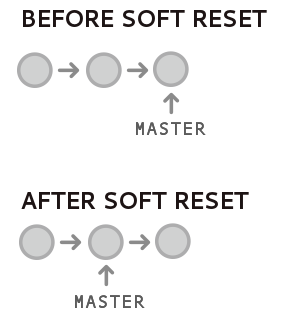
\includegraphics[height=4cm]{imgs/soft-reset.png}
 \end{center}
\end{itemize}
}

\frame
{
\frametitle{hard reset}
\begin{itemize}
 \item \textbf{hard reset}\\ \indent
 El comando git reset -{}-hard <hash> mueve el puntero de la cabeza al hash del commit que le indiquemos y \textbf{destruye} toda la historia hasta dicho hash.\\
 \begin{center}
    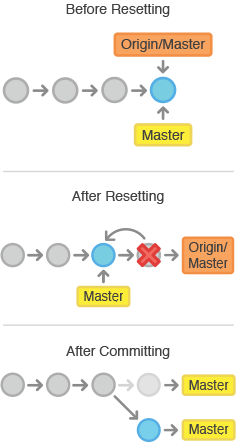
\includegraphics[height=6cm]{imgs/reset-hard.png}
 \end{center}
\end{itemize}
}

\section{Algo más avanzado}
\frame
{
\frametitle{stash}
\begin{itemize}
 \item \textbf{stash}\\ \indent
 Se utiliza para \textit{aparcar} temporalmente los cambios actuales antes de ser comiteados. El comando se escribe únicamente git \textbf{stash}.
 \begin{framed}
 \$ git \textbf{stash} list\\
 stash@\{0\}: WIP on master: 049d078 added the index file\\
 stash@\{1\}: WIP on master: c264051... Revert added file\_size\\
 stash@\{2\}: WIP on master: 21d80a5... added number to log
 \end{framed}
 
 Recuperamos los cambios con el comando git \textbf{stash} apply <id>
\end{itemize}
}

\frame
{
\frametitle{format-patch}
\begin{itemize}
 \item \textbf{format-patch}\\ \indent
 Se utiliza para generar parches que se entregarán a mantenedores de repositorios que no aceptan \textit{pull requests}.\\ \vspace{0.2cm}
 Un parche se genera con el comando git \textbf{format-patch} -{}-stdout \textit{<hash o rango de hashes>}. Esto genera tantos ficheros con parches como commits se hayan introducido como parámetro.\\ \vspace{0.2cm}
 Para aplicar los parches, se utiliza el comando git \textbf{am} -{}-signoff < \textit{file.patch}
\end{itemize}
}

\frame
{
\frametitle{squash}
\begin{itemize}
 \item \textbf{squash}\\ \indent
 Se utiliza dentro de lo que se llama el \textit{rebase interactivo}, para unir varios commits en uno solo antes de entregarlos al repositorio remoto. El proceso sería:
 \begin{itemize}
  \item Comiteamos tantas veces como queramos: git commit -m ``mensaje''
  \item Si por ejemplo hemos hecho 2 commits, ejecutamos el rebase interactivo con: git \textbf{rebase} -i HEAD\textasciitilde2\\ \vspace{0.2cm}
  \footnotesize
   pick 4ca2acc commit file1\\
   pick 7b36971 commit file2\\
   
   \# rebase 41a72e6..7b36971 onto 41a72e6\\
   \#\\
   \# commands:\\
   \#  p, pick = use commit\\
   \#  r, reword = use commit, but edit the commit message\\
   \#  e, edit = use commit, but stop for amending\\
   \#  s, squash = use commit, but meld into previous commit\\
   \#  f, fixup = like ``squash'', but discard this commit's log message\\
   \#  x, exec = run command (the rest of the line) using shell
 \end{itemize}
\end{itemize}
}

\frame
{
\frametitle{squash}
\begin{itemize}
 \item cherry-pick
 \item reflog 
 \item submodules
 \item lolcommits 
\end{itemize}
}